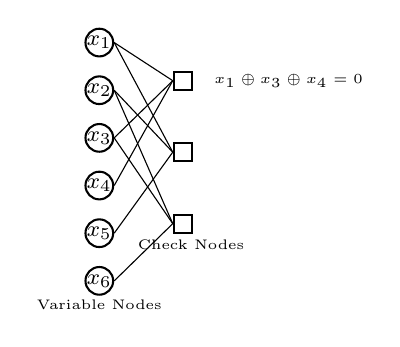
\begin{tikzpicture}
\def\horzgap{7ex}; %Horizontal gap between nodes/levels
\def \gapVN{4ex}; %vertical gap between variable nodes
\def \gapCN{6ex}; %Horizontal gap between check nodes
\def\nodewidth{1.5ex};

\def \textoffs{1ex}; %Offset for writing text east of a node
%\def\nodewidthA{0.05in};
%\def \edgewidth{0.02in};
%\def\ext{0.2in};
`
\def \n{8};
\def\ldeg{2};
\def \m {4};
\def\rdeg{3};

\def\langle{40};%120 degrees/3
\def\langle{20};%120 degrees/6

\tikzstyle{check} = [rectangle, draw, line width=0.75pt, inner sep=0mm, minimum height=\nodewidth, minimum width=\nodewidth]
\tikzstyle{bit} = [circle, draw,line width=0.75pt, inner sep=0mm, minimum size=\nodewidth]

                          
\foreach \vn in {1,...,6}{
 \node[bit] (vn\vn) at (0,-\vn*\gapVN) {\footnotesize $x_{\vn}$};
}


\foreach \cn in {1,...,3}{
\node[check] (cn\cn) at (\horzgap,-0.2*\gapCN-\cn*\gapCN) {};
}

\path (cn1.east)++(\textoffs,0) node ()[anchor=west] {\tiny{$x_1\oplus x_3\oplus x_4=0$}};

%\draw (vn6.east)--(cn4.west);
%\draw (vn3.east)--(cn4.west);
%\draw (vn1.east)--(cn4.west);

%\draw(vn2.east)--(cn3.west);
%\draw (vn4.east)--(cn3.west);
%\draw(vn5.east)--(cn3.west);

\draw (vn2.east)--(cn3.west);
\draw (vn3.east)--(cn3.west);
\draw  (vn6.east)--(cn3.west);

\draw (vn1.east)--(cn2.west);
\draw (vn2.east)--(cn2.west);
\draw (vn5.east)--(cn2.west);

\draw (vn1.east)--(cn1.west);
\draw (vn3.east)--(cn1.west);
\draw (vn4.east)--(cn1.west);

\node () at (0,-6.5*\gapVN){\tiny Variable Nodes};
\node () at (1.1*\horzgap,-3.5*\gapCN){\tiny Check Nodes};

\end{tikzpicture}